\chapter{Introduction to TAO}
\label{chapter:introduction}

% Very introductory, gentle introduction. Pretty tables and figures.
% Perhaps use preamble of \ref{chapter:Getting Started}
% Written in C, but good with C++ compilers.  Also can use fortran.

The Toolkit for Advanced Optimization (TAO) focuses on the design and
implementation of optimization software for the
solution of large-scale optimization applications on high-performance
architectures.  Our approach is motivated by the scattered support for
parallel computations and lack of reuse of linear algebra software in
currently available optimization software.  The TAO design allows the
reuse of toolkits that provide lower-level support (parallel sparse
matrix data structures, preconditioners, solvers), and thus we are
able to build on top of these toolkits instead of having to redevelop
code. The advantages in terms of efficiency and development time are
significant.

The TAO design philosophy uses object-oriented techniques of data and
state encapsulation, abstract classes, and limited inheritance to
create a flexible optimization toolkit.  This chapter provides a short
introduction to our design philosophy by describing the objects in TAO
and the importance of this design. 

\begin{comment}   
 Since a major concern in the TAO
project is the performance and scalability of optimization algorithms
on large problems, we also present some performance resuls.


\end{comment}

\section{TAO Design Philosophy} 

%Use MPI, Microkernal 
% Goals, Current state of art. AD support
%\section{} Use matrices, vectors, linear solvers, as TAO objects

The TAO design philosophy place strongs emphasis on the reuse of
external tools where appropriate.  Our design enables bidirectional
connection to lower-level linear algebra support (e.g. parallel sparse
matrix data structures) provided in toolkits such as PETSc
\cite{petsc} \cite{petsc-user-ref,petsc-web-page}
as well as higher-level application
frameworks.  Our design decisions are strongly motivated by the
challenges inherent in the use of large-scale distributed memory
architectures and the reality of working with large and often poorly
structured legacy codes for specific applications.  Figure
\ref{tao:design} illustrates how the TAO software works with external
libraries and application code.

%\begin{figure}[ht]
%\centering{\includegraphics[height=3.5in,clip]{taofig.eps}}
%\caption{TAO Design}
%\label{tao:design}
%\end{figure}

\begin{figure}
\centerline{\epsfysize=3.5in \epsfbox{taofig.eps}}
\caption{TAO Design}
\label{tao:design}
\end{figure}


The TAO solvers use fundamental PETSc objects to define and solve
optimization problems: vectors, index sets, matrices, and linear
solvers.  The concepts of vectors and matrices are standard, while an
index set refers to a set of integers used to identify particular
elements of vectors or matrices.  An optimization algorithm is a
sequence of well defined operations on these objects.  These
operations include vector sums, inner products, and matrix-vector
multiplication.

With sufficiently flexible abstract interfaces, TAO can support a
variety of implementations of data structures and algorithms.  These
abstractions allow us to more easily experiment with a range of
algorithmic and data structure options for realistic problems, such as
within this case study.  Such capabilities are critical for making
high-performance optimization software adaptable to the continual
evolution of parallel and distributed architectures and the research
community's discovery of new algorithms that exploit their features.

Our current TAO implementation uses the parallel system
infrastructure and linear algebra objects offered by PETSc,
which uses MPI \cite{using-mpi} for all interprocessor communication.
The PETSc package supports objects for vectors, matrices, index 
sets, and linear solvers.

The TAO design philosophy eliminates some of the barriers in using
independently developed software components by accepting data that is
independent of representation and calling sequence written for
particular data formats.  The user can initialize an application with
external frameworks, provide function information to a TAO solver, and
call TAO to solve the application problem.

\section{Changes for Version 2.0}
There are many new features and interface changes that have been introduced
in TAO Version 2, any TAO applications created for previous version will 
need to be updated
to work with the new version.  We apologize for the inconvenience this 
may cause, but we strongly feel that these changes needed to be made
to keep the interface clean, clear, and easy to use. Some of the most
important changes are highlighed in this section.

\subsection{New Algorithms}
One new addition to TAO 2.0 is a new algorithm for solving derivative-free
 nonlinear
least square problems, POUNDerS,
that can efficiently solve parameter optimization problems when no
derivates are available and function evaluations are expensive 
See Section~\ref{sec:pounders} for more information on the details of the
algorithm and Section~\ref{sec:leastsquares} for how to use this algorithm.

TAO 2.0 provides another new algorithm, Linearly Constrained Lagrangian (LCL),
for the solution of PDE-constrained optimization applications.  More information
on PDE-constrained optimization and LCL can be found in Section~\ref{sec:lcl}.

\subsection{Closer Relationship with PETSc}
TAO 2.0 features a tighter association with PETSc styles and practices.
All TAO constructs now follow PETSc conventions are are written in C.
There is no longer a separate abstract class for vectors, matrices, and linear
solvers, TAO now uses these PETSc objects directly. We believe these changes
make TAO applications much easier to create and maintain for users already 
familiar with PETSc programming. These changes also allow TAO to relax some
of the previously imposed requirements on PETSc configuration. TAO can now
work with PETSc configured with single-precision arithmetic, quad-precision 
arithmnetic when using GNU compilers, and no longer requires a C++ compiler.
However, TAO is still not compatible with PETSc installations using complex
data types.

\subsection{Elimination of TaoApplication object}
The largest change to the TAO programming interface is the elimination of the
TaoApplication data structure. In previous versions of TAO, this
structure was created by the application programmer for application-specific
data and routines. However, we now feel that it is clearer and more
closely follows PETSc design principles if this information is directly
attached to a TaoSolver object instead. Please see 
Figure~\ref{fig:tao_commands} for a listing of what the most common TAO 
routines now look like without the TaoApplication object.

\subsection{TaoLineSearch object}
TAO 2.0 features the promotion of line search structures to a full PETSc 
class. This means that any of the available TAO line search algorithms (Armijo, 
Mor\'e-Thuente, GPCG, and unit) can now be selected regardless of the 
overlying TAO algorithm, and it now possible
for a user to create a new line search algorithm that may be more suitable 
for a particular application.  More information on this is available in
Section~\ref{sec:TaoLineSearch}.

\begin{comment}
\section{Performance Results}

A major concern in the TAO project is the performance and scalability
of optimization algorithms on large problems.  In this section we
focus on the GPCG (gradient projection, conjugate gradient) algorithm
for the solution of bound-constrained convex quadratic programming
problems.  Originally developed by Mor\'e and Toraldo
\cite{more-toraldo}, the GPCG algorithm was designed for large-scale
problems but had only been implemented for a single processor.  GPCG
combines the advantages of the identification properties of the
gradient projection method with the finite termination properties of
the conjugate gradient method.  Moreover, the performance of the
TAO implementation on large optimization problems is noteworthy.

%\begin{figure}[tb]
%\centering{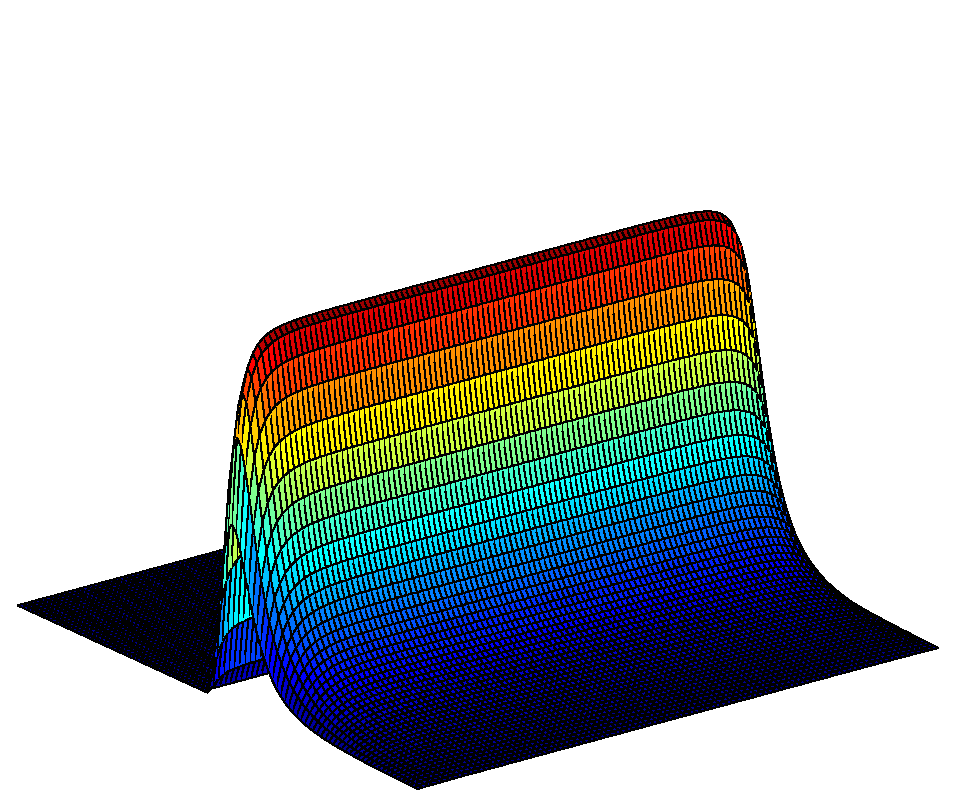
\includegraphics[height=3.0in]{pjb.eps}}
%\caption{The journal bearing problem with $\epsilon$ = 0.9}
%\label{dpjb}
%\end{figure}

\begin{figure}[tb]
\centerline{\epsfysize=3.0in \epsfbox{pjb.eps}}
\caption{The journal bearing problem with $\epsilon$ = 0.9}
\label{dpjb}
\end{figure}



We illustrate the performance of the GPCG algorithm by 
presenting results for a journal bearing problem
with over 2.5 million variables.
The journal bearing problem
is a finite element approximation to a variational problem 
over a rectangular two-dimensional grid.  A
grid with $1600$ points in each direction, for example, is formulated
as a bound constrained quadratic problem with $1600^2=2,560,000$
variables.
The triangulation of the grid results in a matrix that has the
usual five diagonal nonzero structure that arises
from a difference approximation to the Laplacian operator.
The journal bearing problem contains an eccentricity parameter,
$\varepsilon \in (0,1)$, that influences the number of active
variables at the solution and the difficulty in solving it.
Figure \ref{dpjb} shows the solution of the journal bearing problem
for $ \varepsilon = 0.9 $. The steep gradient in the solution
makes this problem a difficult benchmark.

The performance results in Table \ref{flops} are noteworthy is several
ways.  First of all, the number of faces visited by GPCG is remarkably
small.  Other strategies can lead to a large number of gradient
projection iterates, but the GPCG algorithm is remarkably efficient.
Another interesting aspect of these results is that due to the low
memory requirements of iterative solvers, we were able to solve these
problems with only $ p = 8 $ processors.  Strategies that rely on
direct solvers are likely to need significantly more storage, and thus
more processors.  Finally, these results show that the GPCG
implementation has excellent efficiency.  For example, the efficiency
of GPCG with respect to $ p = 8 $ processors ranges between $ 70\% $
and $ 100\% $ when $ \varepsilon = 0.1 $.  This sustained efficiency
is remarkable since the GPCG algorithm is solving a sequence of linear
problems with a coefficient matrix set to the submatrix of the Hessian
matrix with respect to the free variables for the current iterate.
Thus, our implementation's repartitioning of submatrices effectively
deals with the load-balancing problem that is inherent in the GPCG
algorithm.

\begin{table}[htb]
\begin{center}
\begin{tabular}{| c r | c c r c r |}
\hline
\multicolumn{1}{|c}{$ \varepsilon $} & 
\multicolumn{1}{c|}{$ p $} & 
\multicolumn{1}{c}{faces} &
\multicolumn{1}{c}{$n_{CG}$} & 
\multicolumn{1}{c}{time} &
\multicolumn{1}{c}{$t_{CG}$\%} & 
\multicolumn{1}{c|}{$ \cal E $} \\ \hline
0.1  & 8 & 46 & 431 & 7419 & 86 & 100  \\ 
0.1  & 16 & 45 & 423 & 3706 & 83 & 100  \\
0.1  & 32 & 45 & 427 & 2045 & 82 & 91 \\
0.1  & 64 & 45 & 427 & 1279 & 82 & 73 \\
\hline
0.9  & 8 & 37 & 105 & 2134 & 70 & 100 \\
0.9  & 16 & 37 & 103 & 1124 & 71 & 95 \\
0.9  & 32 & 38 & 100 & 618 & 69 & 86 \\
0.9  & 64 & 38 & 99 & 397 & 68 & 67 \\
\hline
\end{tabular}
\caption{Performance of GPCG on the journal bearing problem
with $ 2.56 \cdot 10^6 $ variables.}
\label{flops}
\end{center}
\end{table}




An important aspect of our results that is not
apparent from Table \ref{flops} is that 
for these results we were able to experiment easily 
with all the preconditioners offered by PETSc.
In particular, we were able to compare the diagonal Jacobi
preconditioner with block Jacobi and overlapping additive Schwarz
preconditioners that use a zero-fill ILU solver in each block.  We
also experimented with a parallel zero-fill incomplete Cholesky preconditioner
provided by a PETSc interface to the BlockSolve95~\cite{bs-user-ref}
package of Jones and
Plassmann.  Interestingly enough, the diagonal Jacobi preconditioner
achieved better performance on this problem.



%%% Local Variables: 
%%% mode: latex
%%% TeX-master: "manual_tex"
%%% End: 
\end{comment}
